\documentclass[../main]{subfiles}

\pgfplotsset{every axis/.append style={
                    axis x line=middle,    % put the x axis in the middle
                    axis y line=middle,    % put the y axis in the middle
                    axis line style={<->}, % arrows on the axis
                    xlabel={$x$},          % default put x on x-axis
                    ylabel={$y$},          % default put y on y-axis
                    }}
\tikzset{>=stealth}

\begin{document}

\section{Assumed Knowledge}

\subsection{Algebra}

	\subsubsection{Completing the Square}
	\[ x^2+bx+c = (x+\frac{b}{2})^2+c-(\frac{b}{2})^2 \]
	\subsubsection{Polynomial Expansions}
	\begin{equation*} \begin{gathered}
		(a\pm b)^2 = a^2 \pm 2ab + b^2 \\
		a^2 - b^2 = (a+b)(a-b) \\
		a^3 \pm b^3 = (a \pm b)(a^2 \mp ab + b^2)
	\end{gathered} \end{equation*}
	\subsubsection{Partal Fractions}
	\begin{equation*} \begin{gathered}
		\frac{f(x)}{(ax+b)(cx+d)} \\ = g(x) + \frac{A}{ax+b} + \frac{B}{cx+d} \\
		\frac{f(x)}{(ax+b)(cx+d)^2} \\ = g(x) + \frac{A}{ax+b} + \frac{B}{cx+d} + \frac{C}{(cx+d)^2} \\
		\frac{f(x)}{(ax+b)(x^2+c)} \\ = g(x) + \frac{A}{ax+b} + \frac{Bx+C}{x^2+c}
	\end{gathered} \end{equation*}
	\subsubsection{Exponent and Logarithm}
	\begin{equation*} \begin{gathered}
		e^n = \underbrace{e \times e \times e \times ... \times e}_\text{n times} \\
		e^\frac{1}{2} = \sqrt{e} \\
		\log_{e}(x) = \ln(x) \\ = \text{how many times \(e\) is multiplied by itself to get x} \\
		\log_{10}(x) = \lg(x) \\
		x = e^{ln(x)} \\
		\log_x(y) = \frac{\log_{base}(y)}{\log_{base}(x)} 
	\end{gathered} \end{equation*}
	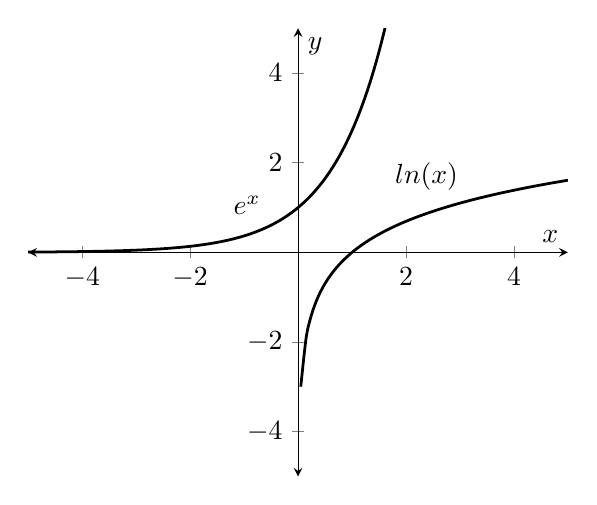
\begin{tikzpicture} \begin{axis}[domain=-5:5,ymin=-5,ymax=5,samples=100,mark=none,smooth]
	    \addplot[color=black,no marks,line width=1pt,-] {e^x} node[pos=0.03,anchor=south east]{$e^x$};
	    \addplot[color=black,no marks,line width=1pt,-] {ln(x)} node[pos=0.75,anchor=south east]{$ln(x)$};  
	\end{axis} \end{tikzpicture}

\subsection{Trigonometry}
	
	\subsubsection{Sine and Cosine Rule}
	For any triangle with length of sides \(a\), \(b\) and \(c\) and with opposite angles \(A\) \(B\) and \(C\):
	\begin{equation*} \begin{gathered}
		\frac{a}{\sin(A)}=\frac{b}{\sin(B)}=\frac{c}{\sin(C)} \\
		a^2 = b^2 + c^2 - 2 b c \cos(A) \\
		\cos(A) = \frac{b^2 + c^2 - a^2}{2bc}
	\end{gathered} \end{equation*}
	\subsubsection{Sum of Angles}
	\begin{equation*} \begin{gathered}
		\sin(A \pm B) = \sin(A)\cos(B) \pm \cos(A)\sin(B) \\
		\sin(2A) = 2\sin(A)\cos(A) \\
		\cos(A \pm B) = \cos(A)\cos(B) \mp \sin(A)\sin(B) \\
	\end{gathered} \end{equation*}
	\begin{equation*} \begin{split}
		\cos(2A) & = \cos^2(A) - \sin^2(A) \\
				& = 2\cos^2(A) - 1 \\
				& = 1 - 2\sin^2(A)
	\end{split} \end{equation*}
	\begin{equation*} \begin{gathered}
		\tan(A \pm B) = \frac{\tan(A) \pm \tan(B)}{1 \mp \tan(A)\tan(B)} \\
		\tan(2A) = \frac{2\tan(A)}{1-\tan^2(A)} 
	\end{gathered} \end{equation*}
	\[ \text{Area of Triangle} = \tfrac{1}{2}absin(C) \]
	\subsubsection{Factor and Reverse Factor Formula}
	\begin{equation*} \begin{gathered}
		\sin(A)+\sin(B) = 2\sin(\tfrac{A+B}{2})\cos(\tfrac{A-B}{2}) \\
		\sin(A)-\sin(B) = 2\cos(\tfrac{A+B}{2})\sin(\tfrac{A-B}{2}) \\
		\cos(A)+\cos(B) = 2\cos(\tfrac{A+B}{2})\cos(\tfrac{A-B}{2}) \\
		\cos(A)-\cos(B) = -2\sin(\tfrac{A+B}{2})\sin(\tfrac{A-B}{2}) \\
		\sin(A)\cos(B) = \tfrac{1}{2} [ \sin(A+B) + \sin(A-B) ] \\
		\cos(A)\sin(B) = \tfrac{1}{2} [ \sin(A+B) - \sin(A-B) ] \\ 
		\cos(A)\cos(B) = \tfrac{1}{2} [ \cos(A+B) + \cos(A-B) ] \\
		\sin(A)\sin(B) = -\tfrac{1}{2} [ \cos(A+B) - \cos(A-B) ]
	\end{gathered} \end{equation*}

	Factor formulae are given in MF10. Reverse factor formula can be derived using factor formula.

	\begin{center} \begin{tikzpicture}
	\draw (0,1) node[anchor=south] {\(\sin(A)+\sin(B) = 2\sin(\tfrac{A+B}{2})\cos(\tfrac{A-B}{2})\)};
	\draw (0,0) node[anchor=north] {\(\tfrac{1}{2} [ \sin(X+Y) + \sin(X-Y) ] = \sin(X)\cos(Y)\)};
	\draw [->] (0,1) -- (-3.4,0) ;
	\draw [->] (-2.2,1) -- (-2,0) ;
	\draw [->] (-0.7,1) -- (0.1,0) ;
	\draw [->] (1.1,1) -- (2.2,0) ;
	\draw [->] (2.6,1) -- (3.2,0) ;
	\end{tikzpicture} \end{center}

\end{document}